\section{Exercise 1: Basic implementation of the Hopfield network}
\subsection{1.1 Getting started}

\begin{itshape}
\small
Asynchronous updating of the nodes ensures that the dynamics of the Hopfield model with symmetric weights $w_{ij} = w_{ji}$ always converge to a fixed point. An energy function in this case is given by:
\begin{equation}
H(t)=-\sum_{i=1}^n \sum_{j=1}^n \omega_{ij} S_i(t) S_j(t)
\label{eq: energy function}
\end{equation}
Implement the Hopfield network as described above. Shortly comment on your implementation. The overlap of the network in state $S(t)$ with a given pattern $\xi^{\mu}$ is defined by $\frac{1}{N}\sum_{i=1}^N \xi_i^{\mu} 	S_i(t)$. Set $N = 200$, $P = 5$, $c = 0.2$. For the first two unit time steps of the retrieval of one pattern, plot the changing values of the energy function and the overlap of the network with the pattern as the state of each node is sequentially updated.
\end{itshape}

\begin{wrapfigure}{r}{0.5\textwidth}
  \vspace{-42pt}
  \begin{center}
    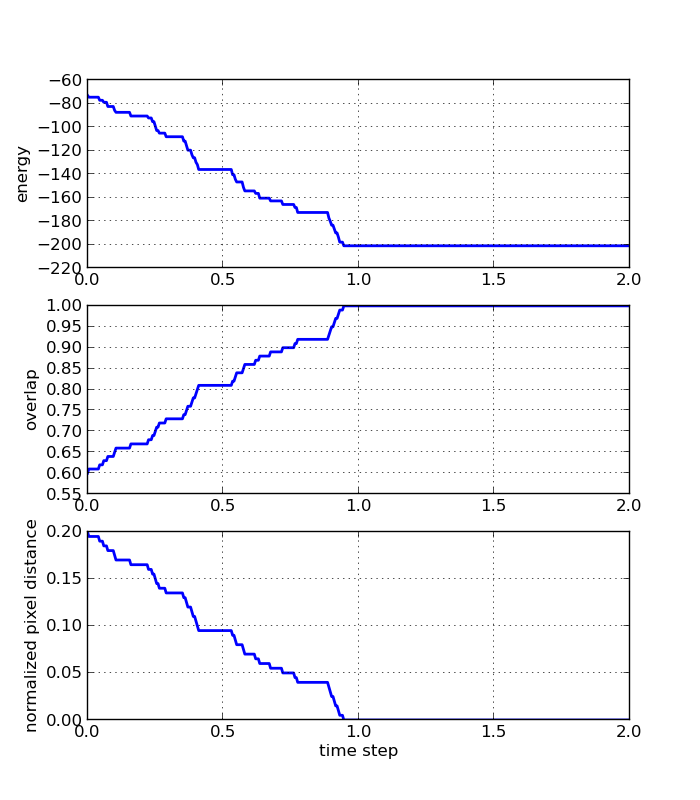
\includegraphics[width=0.5\textwidth]{dat/ex1_1-energy_overlap-N200-P5-c20}
  \end{center}
  \vspace{-20pt}
  \caption{Exercise 1	}
  \label{fig: Question 1.1}
  \vspace{-10pt}
\end{wrapfigure}

\paragraph*{}

The Hopfield Network works by taking one of the $P$ patterns stored in the system with the index $\mu$ and flipping a certain percentage \texttt{flip$\_$ratio} of its pixels. The resulting pattern is then used as the pattern that is to be tested and the dynamics are run on that pattern. 
In order to execute the source code of the Hopfield Network, one should first execute \texttt{h=HopfieldNetwork()} in order  to initialize the class. Then one can execute the class using \texttt{h.run()}. The  options of the \texttt{run} function are \texttt{N} (number of pixels), \texttt{P}  (number of patterns), \texttt{ratio} (fraction of $\xi_i=1$ in patterns), \texttt{mu} (pattern  chosen for modification and subsequent retrieval), \texttt{flip$\_$ratio} (fraction of pixels that are to be  changed when creating the retrieval pattern), \texttt{pcut} (the probability that a directed weight $\omega_{ij}$ is cut and set to 0), \texttt{excitatory} (sets disallowed connection weights in standard Hebbian to 0),\texttt{bPlot} (whether  a plot should be created) and \texttt{bDebug} (whether debugging tools should be turned  on).

In figure \ref{fig: Question 1.1} the dynamics needed to retrieve the pattern with the above given settings are shown. The image shows the energy, the overlap and the normalized pixel distance which is explained in section \ref{ssec: Normalized Pixel Distance}. Not even one complete time-step was necessary in order to retrieve the pattern with a 100$\%$ overlap. During the retrieval, the energy function fell strongly, showing that we were approaching a stable condition. 
\paragraph*{}
At first, the script only ran very slowly, this is because we did not have a lot of  experience with python and thus used to for loops to do matrix multiplications. After  implementing the \texttt{numpy.dot} function, the script ran incredibly much faster. 

\subsection{1.2 Normalized Pixel Distance}
\label{ssec: Normalized Pixel Distance}
\begin{itshape}
\small
Using the overlap defined in 1.1, derive an expression for the percentage of pixels in the network state $S$ which differ from the pattern $\xi^\mu$. This is the (normalized) pixel distance.
\end{itshape}

\paragraph*{}

The overlap gives the fraction of pixels which are identical between the network in state $S(t)$ and the pattern $\xi^\mu$. Because the Normalized Pixel Distance (NPD) must be in the domain $[0,1]$, it must be given by:

\begin{equation}
d=\frac{1- \frac{1}{N} \sum_{i=1}^N \xi_i^{mu} S_i(t)}{2}
\end{equation}

A NPD of 0 indicates that the two pattern are identical, a NPD of 1 indicates that the two patterns are the inverse of each other. The normalized pixel distance was plotted together with the energy and the overlap in figure \ref{fig: Question 1.1}.

\subsection{1.3 Pattern retrieval}

\begin{itshape}
\small
We define the retrieval error of a pattern $\xi^\mu$ in a Hopfield network as the normalized pixel distance of the network state $S$ to the pattern $\xi^\mu$ after convergence, when retrieving the pattern $\xi^\mu$ as described above.

Set N = 200 and c = 0.1. Plot the mean retrieval error of a randomly chosen pattern averaged over different network realizations as a function of the dictionary size P. Average over enough network realizations to give a smooth curve and give error bars for the estimation of the mean (you can assume the variation to be normally distributed). From your data points and the chosen confidence interval, roughly estimate a maximal P at which patterns can be retrieved from the network with a mean retrieval error of less than 2$\%$?

\end{itshape}

\begin{figure}
  \vspace{-20pt}
  \begin{center}
    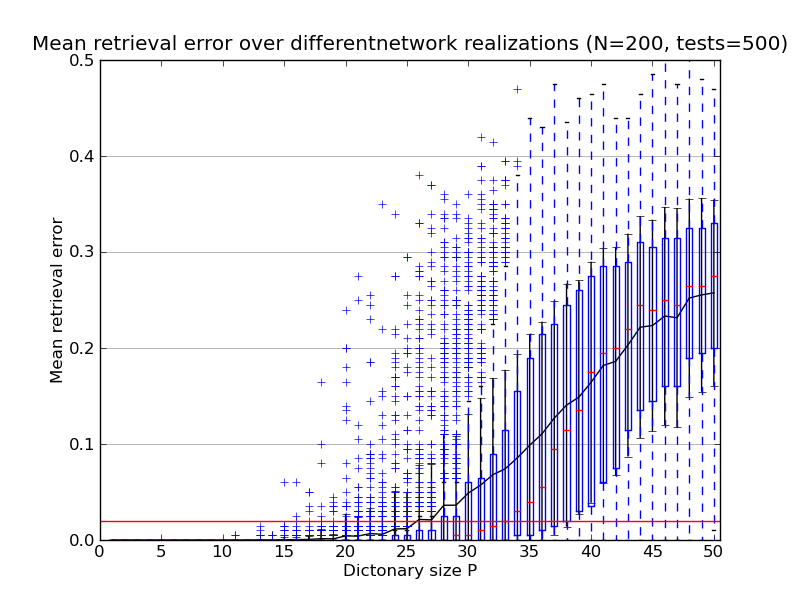
\includegraphics[width=0.9\textwidth]{dat/ex1_3-error_avg-N200-P50-Q500.png}
  \end{center}
  \vspace{-20pt}
  \caption{Exercise 1.3: Mean retrieval error averaged over 500 different network realizations.}
  \label{fig: Question 1.3}
  \vspace{-10pt}
\end{figure}

\paragraph*{}

Figure \ref{fig: Question 1.3} shows a plot of the mean retrieval error with respect to the dictionary size P averaged over 500 network iterations. The error remains approximately 0 up to a dictionary size of $P=20$. It then starts mounting quickly and already reaches 25$\%$ at $P=50$. The horizontal red line indicates the 2$\%$ threshold. It is reached at $P=26$. In the plot, the blue box depicts the data between the lower and the upper quartile of errors, the extremities of the dotted line depict the end of the data and the blue crosses indicate runaway values. The black error plot indicates the $1\sigma$ interval and the red line in the boxes indicates the median value of the errors. The black plot is the graph of the mean retrieval error. 

